% Standalone write-up of the DMFT for the scale-invariant (relative) GLV.
% Compiles on its own (pdflatex -> biber -> pdflatex x2) and reuses thesis/bib.bib.
% To fold into the thesis: delete the preamble down to \begin{document}, the title block,
% and the closing \printbibliography/\end{document}, then \include this as a chapter.
\documentclass{report}
\usepackage{graphicx}
\usepackage{amsmath}
\usepackage{amssymb}
\usepackage{placeins}
\usepackage{hyperref}
\usepackage[natbib=true]{biblatex}
\addbibresource{bib.bib}

\newcommand{\Dz}{\mathcal{D}z}
\newcommand{\E}{\mathbb{E}}

\begin{document}

\begin{center}
{\Large\bfseries A dynamical mean-field theory for the scale-invariant GLV}\\[4pt]
{\itshape Ludovico Furlanetto}\\[2pt]
\today
\end{center}
\vspace{0.6cm}

This note derives a dynamical mean-field theory (DMFT) for the scale-invariant model of
the growing-economy chapter, in which the interactions act on the average firm rather
than on absolute abundances. The model turns out to be a disordered replicator equation,
so its DMFT is the heterogeneous single-site process already used to locate $\mu_c$
\citep{aguirrelopez}, with two small additions that the scale invariance forces. The
resulting fixed-point theory predicts the relaxed-to-fluctuating boundary, the survival
fraction and the aggregate growth rate in closed form, and a direct simulation on the
matching graph confirms it to about one percent with no fitting.

\section{The model and its reduction to a replicator}
\label{sec:dmft-model}

We take the relative GLV in the competition convention used in the simulations,
\begin{equation}
    \dot x_i = x_i\left[\,1 - \frac{x_i}{m} - \frac{(\alpha x)_i}{m}\,\right],
    \qquad m = \frac1N\sum_j x_j = \frac MN ,
    \label{eq:dmft-glv}
\end{equation}
with couplings on a graph of mean degree $C$,
\begin{equation}
    \alpha_{ij} = A_{ij}\Big(\frac{\mu}{C} + \frac{\sigma}{\sqrt C}\,z_{ij}\Big),\qquad
    z_{ij}\sim\mathcal N(0,1),\qquad \overline{z_{ij}z_{ji}} = \gamma,\qquad \alpha_{ii}=0 .
\end{equation}
Both the self-limitation $x_i/m$ and the interaction $(\alpha x)_i/m$ are divided by the
population mean $m$. The right-hand side of \eqref{eq:dmft-glv} is then homogeneous of
degree one in $x$, so the bracket $F_i := 1 - x_i/m - (\alpha x)_i/m$ depends on $x$ only
through ratios. The overall scale is a free direction that grows or decays exponentially
without the finite-time blow-up of the absolute model.

Introduce the relative abundances $y_i = x_i/m$, which satisfy $\langle y\rangle :=
\frac1N\sum_i y_i = 1$ by construction, and let $M = \sum_j x_j$ be the total. The
aggregate grows at the population-averaged fitness,
\begin{equation}
    g(t) := \frac{d\ln M}{dt}
          = \frac1M\sum_j \dot x_j = \sum_j \frac{x_j}{M}\,F_j
          = \frac1N\sum_j y_j F_j = \langle yF\rangle .
    \label{eq:dmft-g}
\end{equation}
Subtracting this common scale leaves a closed equation for the relative abundances,
\begin{equation}
    \dot y_i = y_i\big(F_i - g(t)\big),\qquad
    F_i = 1 - y_i - (\alpha y)_i,\qquad
    g(t) = \langle yF\rangle ,
    \label{eq:dmft-replicator}
\end{equation}
which is a replicator equation, the simplex projection of \eqref{eq:dmft-glv} in the sense
of Hofbauer's correspondence \citep{hofbauer81}. The aggregate is recovered from
$M(t) = M(0)\exp\!\int_0^t g$, and a positive stationary $g$ is a steadily growing
economy.

\paragraph{What the $-g(t)$ term is.}
The drift $-g(t)$ in \eqref{eq:dmft-replicator} is the mean-fitness subtraction of the
replicator, and it is the term that turns the equation for absolute size into one for
relative size. From \eqref{eq:dmft-g}, $g(t) = \langle yF\rangle = \sum_j w_j F_j$ is the
share-weighted average fitness of the whole economy, with shares $w_j = y_j/N = x_j/M$,
and it equals the growth rate of the aggregate, $g(t) = d\ln M/dt$. Every firm feels the
same $g(t)$: it is a global field, not something private to firm $i$. A firm therefore
gains relative size, $\dot y_i > 0$, only when its own fitness $F_i$ exceeds the
economy-wide average $g(t)$, so $-g(t)$ encodes the requirement to beat the field in
order to gain ground. Its role is to enforce the constraint $\langle y\rangle = 1$: one
checks from \eqref{eq:dmft-replicator} that $\frac{d}{dt}\langle y\rangle = \langle
yF\rangle - g\langle y\rangle = g\,(1 - \langle y\rangle)$, so $\langle y\rangle = 1$ is
preserved, and $g(t) = \langle yF\rangle$ is precisely the value that keeps it preserved.
Because it is an average over the whole population, $g(t)$ self-averages: its fluctuations
are of order $1/\sqrt N$ and vanish in the thermodynamic limit, so it enters the mean-field
description as a deterministic common drift rather than as a source of noise.

\section{The local field and the effective single-site process}
\label{sec:dmft-cavity}

We take the high-connectivity limit and treat the regular graph first, so that
$k_i \equiv C$; the degree-heterogeneous case is recovered in
Section~\ref{sec:dmft-outlook}. Split the interaction felt by node $i$ into its mean and
its fluctuation,
\begin{equation}
    (\alpha y)_i
    = \frac{\mu}{C}\sum_{j\in\partial i} y_j + \frac{\sigma}{\sqrt C}\sum_{j\in\partial i} z_{ij} y_j
    \;\longrightarrow\; \mu M_1(t) + h_i(t),
\end{equation}
where the neighbourhood average of the mean part tends to the global one, $\mu M_1$ with
$M_1 = \langle y\rangle$, and $h_i$ collects the disorder. The dynamical cavity argument
\citep{bunin2017,galla2018} proceeds by removing node $i$: the cavity trajectories
$y_j^{(i)}$ are independent of the couplings $\{z_{ij}, z_{ji}\}$, and reinstating $i$
perturbs each neighbour by linear response. The field that $i$ exerts on $j$ has
fluctuating part $-\frac{\sigma}{\sqrt C} z_{ji} y_i$, so with the single-site response
$G_j(t,s) = \delta y_j(t)/\delta\zeta_j(s)$,
\begin{equation}
    h_i(t)
    = \frac{\sigma}{\sqrt C}\sum_{j\in\partial i} z_{ij}\,y_j^{(i)}(t)
    \;-\; \frac{\sigma^2}{C}\sum_{j\in\partial i} z_{ij}z_{ji}\!\int_0^t\! ds\,G_j(t,s)\,y_i(s).
\end{equation}
The first sum is a sum of $C$ independent zero-mean terms; by the central limit theorem it
becomes a Gaussian noise $\xi_i(t)$ whose covariance is the population autocorrelation,
\begin{equation}
    \langle\xi_i(t)\xi_i(s)\rangle
    = \frac{\sigma^2}{C}\sum_{j\in\partial i} y_j(t)y_j(s)
    = \sigma^2\,C(t,s),\qquad C(t,s):=\langle y(t)y(s)\rangle .
\end{equation}
The second sum uses $\overline{z_{ij}z_{ji}} = \gamma$ and
$\frac1C\sum_{j\in\partial i} G_j \to G := \langle G_j\rangle$, giving the retarded Onsager
reaction $-\gamma\sigma^2\!\int_0^t G(t,s)\,y_i(s)\,ds$. Substituting into $F_i = 1 - y_i -
\mu M_1 - h_i$ and using \eqref{eq:dmft-replicator} produces the effective single-site
process
\begin{equation}
    \boxed{\;
    \dot y = y\left[\,1 - y - \mu M_1(t) - g(t)
        + \sigma\,\eta(t) + \gamma\sigma^2\!\int_0^t\! G(t,s)\,y(s)\,ds\,\right],
    \;}
    \label{eq:dmft-effective}
\end{equation}
with $\eta$ a unit-strength Gaussian noise of covariance $\langle\eta(t)\eta(s)\rangle =
C(t,s)$. Equation~\eqref{eq:dmft-effective} is the heterogeneous effective process of
\citet{aguirrelopez} with carrying capacity $K=1$, the competition sign on the mean field,
and the two structural additions forced by the scale invariance: the common drift $-g(t)$
of Section~\ref{sec:dmft-model}, and the constraint that the mean abundance is pinned,
$M_1\equiv 1$, rather than left free.

\section{Self-consistency}
\label{sec:dmft-selfconsistency}

The disorder average is now carried by four functionals of the single-site law of
\eqref{eq:dmft-effective}:
\begin{equation}
    M_1(t) = \E[y(t)] = 1,\qquad
    C(t,s) = \E[y(t)y(s)],\qquad
    G(t,s) = \E\!\left[\frac{\delta y(t)}{\delta\zeta(s)}\right]_{\zeta=0},
\end{equation}
\begin{equation}
    g(t) = \E[y(t)F(t)],\qquad
    F = 1 - y - \mu M_1 + \sigma\eta + \gamma\sigma^2\!\int_0^t G\,y .
    \label{eq:dmft-closures}
\end{equation}
The first is the normalisation, the middle two are the standard correlation and response
that close the noise and the memory, and the last fixes the common drift. The closure for
$g$ is forced rather than chosen: $\dot M_1 = \E[yF] - g M_1$, and demanding $\dot M_1 = 0$
at $M_1 = 1$ gives $g(t) = \E[yF]$. This is the structure of the solvable random-replicator
model of \citet{diederich1989}, here carrying the GLV self-limitation as well.

\section{The fixed point: the relaxed phase}
\label{sec:dmft-fixedpoint}

In the single-fixed-point phase the shares relax, $y(t)\to y^\ast$, and the statistics
become time-translation invariant. The correlation tends to a constant $C(t,s)\to q :=
\E[y^{\ast 2}]$, so the coloured noise freezes to a static Gaussian $\sigma\eta \to
\sigma\sqrt q\,z$ with $z\sim\mathcal N(0,1)$, and the memory becomes
$\gamma\sigma^2\!\int_0^t G\,y \to \gamma\sigma^2\chi\,y^\ast$ with the static
susceptibility $\chi = \int_0^\infty G(u)\,du$. Setting $\dot y = 0$ in
\eqref{eq:dmft-effective},
\begin{equation}
    y^\ast(z) = \frac{(1 - g^\ast) - \mu M_1 + \sigma\sqrt q\,z}{\,1 - \gamma\sigma^2\chi\,}
    \quad\text{if positive, else } 0 .
    \label{eq:dmft-ystar}
\end{equation}
This is the GLV survivor law \citep{bunin2017,galla2018} with the carrying capacity
renormalised by the growth rate, $K \to 1 - g^\ast$. Writing $v = 1 - \gamma\sigma^2\chi$,
$\Delta = (1 - g^\ast - \mu M_1)/(\sigma\sqrt q)$ and the Gaussian moments $w_n(\Delta) =
\int_{-\Delta}^\infty \Dz\,(\Delta+z)^n$ with $\Dz = e^{-z^2/2}dz/\sqrt{2\pi}$, the
self-consistency conditions for $(\Delta, q, \chi, g^\ast)$ at $M_1\equiv 1$ are
\begin{equation}
    \varphi = w_0(\Delta),\qquad
    \frac{\sigma\sqrt q}{v}\,w_1(\Delta) = 1,\qquad
    v^2 = \sigma^2 w_2(\Delta),\qquad
    \chi = \frac{w_0(\Delta)}{v} .
    \label{eq:dmft-sc}
\end{equation}
These are the fixed-point equations of the absolute model with one extra unknown $g^\ast$
and one extra equation, the normalisation $\tfrac{\sigma\sqrt q}{v} w_1 = 1$, which fixes
it. The growth rate $g^\ast = \langle y^\ast F^\ast\rangle$ is the scale-invariant model's
analogue of the shape scalar used to locate $\mu_c$, and $g^\ast > 0$ marks the growing
region.

\section{Stability and the phase boundary}
\label{sec:dmft-boundary}

The fixed point is linearly stable until the disorder feedback develops a zero mode, at the
marginal condition
\begin{equation}
    \sigma^2\varphi = (1 - \gamma\sigma^2\chi)^2 = v^2 .
    \label{eq:dmft-stability}
\end{equation}
At threshold the mean-square equation $v^2 = \sigma^2 w_2(\Delta)$ then forces $w_0(\Delta)
= w_2(\Delta)$, whose unique root is $\Delta = 0$, so exactly half the species survive
($\varphi = \tfrac12$) and, with $w_2(0) = \tfrac12$,
\begin{equation}
    \sigma_c = \sqrt 2 \qquad (\gamma = 0),
\end{equation}
the standard onset of the high-diversity fluctuating phase \citep{galla2018,roy2020}.
Because $\Delta = 0$ at threshold, $\mu$ and $g^\ast$ drop out of the condition entirely:
on the regular graph the boundary is independent of $\mu$, a horizontal line. This is the
mean-field statement of a fact specific to the relative model. Since $\mu$ enters every
fitness as the same shift $\mu M_1 = \mu$, it cancels in the replicator and cannot change
the relaxed-or-fluctuating structure; it only sets the level of the growth rate, $g^\ast =
g_0 - \mu$, and so moves the $g^\ast = 0$ contour but not the chaos boundary. The left
panel of Figure~\ref{fig:dmft-phase} shows the resulting structure, and the right panel the
$\mu$-independent order parameters: the growth part $g_0(\sigma)$ rises from $0$ to $1$ as
$\sigma\to\sqrt2$, so disorder drives the growth, while the survival fraction
$\varphi(\sigma)$ falls from $1$ to $\tfrac12$ at the onset.

\begin{figure}[htbp]
    \centering
    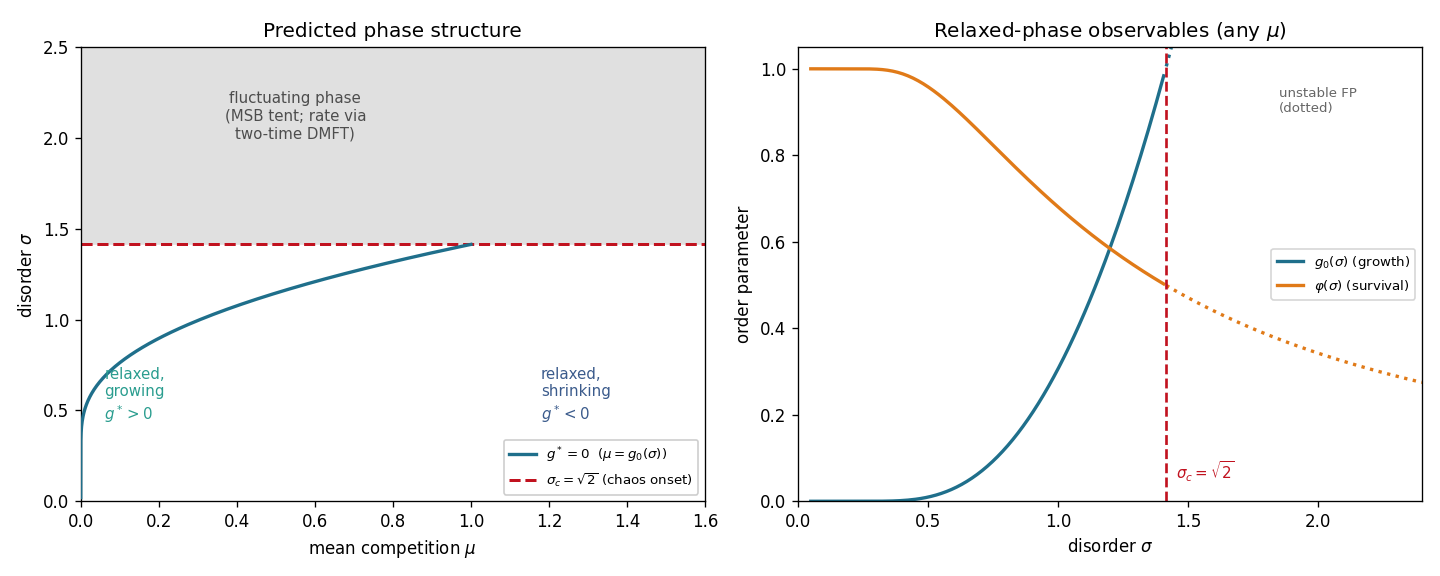
\includegraphics[width=\linewidth]{dmft_phase.png}
    \caption{Phase structure predicted by the solution of
    \eqref{eq:dmft-sc}--\eqref{eq:dmft-stability} at $\gamma=0$. Left: the $(\mu,\sigma)$
    plane. The chaos onset $\sigma_c = \sqrt2$ (red dashed) is horizontal, independent of
    $\mu$; the growth contour $g^\ast = 0$ (blue, $\mu = g_0(\sigma)$) separates the
    relaxed growing region from the relaxed shrinking one. The fluctuating phase above
    $\sigma_c$, where the firm-growth tent lives, needs the two-time theory of
    Section~\ref{sec:dmft-outlook}. Right: the $\mu$-independent order parameters
    $g_0(\sigma)$ and $\varphi(\sigma)$; dotted beyond $\sigma_c$, where the fixed point is
    unstable.}
    \label{fig:dmft-phase}
\end{figure}

\section{What the theory predicts}
\label{sec:dmft-observables}

The fixed-point solution delivers, in closed form and as functions of $(\mu,\sigma)$, the
aggregate growth rate $g^\ast$, the surviving fraction $\varphi$, and the relative-size
distribution $P(y)$ as the pushforward of $\mathcal N(0,1)$ through \eqref{eq:dmft-ystar}.
The boundary \eqref{eq:dmft-stability} is the same curve mapped numerically as the
shape-relaxation line. The size-variance exponent $\beta$, by contrast, is a property of
the fluctuations and so is undefined at the static fixed point, where the shares do not
move; it lives in the fluctuating phase and requires the two-time theory. Its mean-field
character is already visible, however: the noise $\eta$ in \eqref{eq:dmft-effective} is a
single common field, so the single-site description contains no genuine cross-firm
correlation. Any nonzero $\beta$ it produces must therefore come from the single-firm
mechanics, the self-limitation $-y$ and the memory, rather than from correlations between
firms, which is the analytic counterpart of the observation that switching off the disorder
removes the size-variance law \citep{moran2024}.

\section{Numerical validation}
\label{sec:dmft-validation}

The solver of \eqref{eq:dmft-sc}--\eqref{eq:dmft-stability} is tested against a direct
simulation on the matching ensemble: a fully-connected graph with Gaussian couplings
$\alpha_{ij} = \mu/N + (\sigma/\sqrt N) z_{ij}$ at $\gamma = 0$, $N = 1500$, and no
immigration, which is the exact setting of the regular-graph theory. The integration uses
the share-plus-scale split, returns the growth rate $g_{\mathrm{eff}}$ from the slope of
$\ln M$, the surviving fraction, and the late-time amplitude of the share fluctuations.
Table~\ref{tab:dmft-validation} and Figure~\ref{fig:dmft-validation} report the comparison.

\begin{table}[htbp]
    \centering
    \begin{tabular}{rrrrrl}
        \hline
        $\sigma$ & $g_{\mathrm{eff}}$(sim) & $g^\ast$(DMFT) & surv(sim) & $\varphi$(DMFT) & phase \\
        \hline
        0.40 & $-0.494$ & $-0.498$ & 0.991 & 0.989 & relaxed \\
        0.70 & $-0.429$ & $-0.433$ & 0.860 & 0.854 & relaxed \\
        1.00 & $-0.199$ & $-0.195$ & 0.690 & 0.681 & relaxed \\
        1.20 & $+0.061$ & $+0.085$ & 0.601 & 0.585 & relaxed \\
        1.35 & $+0.297$ & $+0.363$ & 0.540 & 0.523 & relaxed \\
        1.60 & $+0.911$ & $+0.959$ & 0.371 & 0.440 & fluctuating \\
        2.00 & $+2.032$ & $+2.272$ & 0.206 & 0.343 & fluctuating \\
        2.50 & $+3.946$ & $+4.551$ & 0.090 & 0.261 & fluctuating \\
        \hline
    \end{tabular}
    \caption{Simulation versus DMFT at $\mu = 0.5$, $\gamma = 0$, $N = 1500$. In the
    relaxed phase ($\sigma < \sqrt2$) the mean discrepancies are $|g_{\mathrm{eff}} -
    g^\ast| = 0.021$ and $|\text{surv} - \varphi| = 0.010$. Beyond $\sigma_c$ the static
    values overshoot, since the fixed point is unstable there.}
    \label{tab:dmft-validation}
\end{table}

\begin{figure}[htbp]
    \centering
    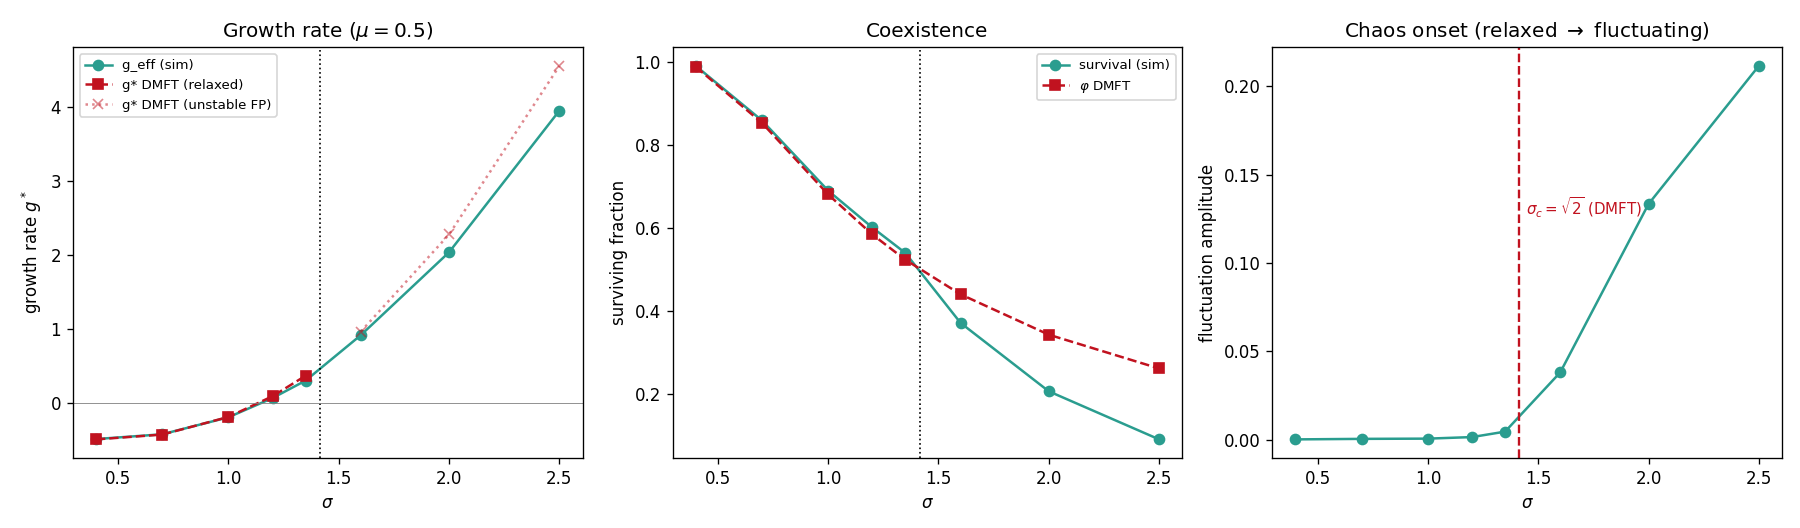
\includegraphics[width=\linewidth]{dmft_validation.png}
    \caption{Direct simulation (teal) against the DMFT (red) on the matched
    fully-connected ensemble, $\mu = 0.5$, $\gamma = 0$, $N = 1500$. Left: the growth rate
    tracks $g^\ast$ in the relaxed phase and the unstable-fixed-point branch (dotted)
    overshoots beyond $\sigma_c$. Centre: the surviving fraction follows $\varphi$ up to
    $\sigma_c$. Right: the persistent-fluctuation amplitude is negligible below
    $\sigma_c = \sqrt2$ and switches on exactly at the predicted onset.}
    \label{fig:dmft-validation}
\end{figure}

Three predictions are confirmed. In the relaxed phase the growth rate and the survival
fraction match to about one to two percent with no fitting. The fluctuation amplitude is
below $0.005$ for $\sigma < \sqrt2$ and jumps to $0.038$, $0.13$ and $0.21$ at $\sigma =
1.6, 2.0, 2.5$, locating the chaos onset at the predicted $\sqrt2$. And the
$\mu$-independence holds exactly: at $\sigma = 1.0$, sweeping $\mu = 0, 1, 2$ leaves the
survival fraction fixed at $0.688, 0.687, 0.685$ and shifts $g_{\mathrm{eff}}$ by exactly
$-\mu$, giving $+0.317, -0.682, -1.681$. Beyond $\sigma_c$ the static $g^\ast$ and
$\varphi$ overshoot the simulation, which is the quantitative signal that the relaxed-phase
theory has run out and the fluctuating phase needs a genuinely dynamical treatment.

\section{Validity and outlook}
\label{sec:dmft-outlook}

The theory is exact for $N\to\infty$ in the high-connectivity limit, the same regime
assumed for $\mu_c$. A node of rescaled degree $\kappa = k/C$ obeys
\eqref{eq:dmft-effective} with $\mu M_1 \to \kappa\mu M_1$, $\sigma \to \sqrt\kappa\,\sigma$
and $\gamma\sigma^2 \to \kappa\gamma\sigma^2$, and the order parameters become averages over
the rescaled degree law $\nu(\kappa)$, with the normalisation taken on the flat node
average. Degree heterogeneity reintroduces the $\mu$ dependence of the boundary that the
regular graph removes. The power-law degree of the production runs has a divergent second
moment $\langle\kappa^2\rangle$, so the regular-graph value $\sigma_c = \sqrt2$ is not
expected to transfer to it quantitatively, and a comparison there should use an exponential
or regular graph.

The relaxed phase studied here is the steadily growing region. The firm-growth tent and the
fat tails live in the fluctuating phase above $\sigma_c$, where the fixed point is unstable
and the two-time correlation and response must be integrated forward
\citep{roy2020,diederich1989}. Computing the size-variance law there, from a single-site
process that by construction contains no cross-firm correlation, is the natural next step
and the one that would settle the origin of $\beta$.

\printbibliography

\end{document}
